% ============================================================================
% CHAPTER 1E: THERMAL AND FLUID SYSTEMS
% ============================================================================

\chapter{Thermal and Fluid Systems}
\label{ch:thermal_fluid}

Thermal and fluid systems are governed by energy and mass conservation. These systems often exhibit first-order dynamics with relatively slow time constants, making them excellent candidates for feedback control.

% ============================================================================
\section{Thermal Systems Fundamentals}
\label{sec:thermal_fundamentals}
% ============================================================================

\subsection{Heat Transfer Mechanisms}

\subsubsection{Conduction (through solids)}
\begin{equation}
\dot{Q} = \frac{kA}{L}(T_1 - T_2) = \frac{T_1 - T_2}{R_{th}}
\end{equation}

where $R_{th} = L/(kA)$ is the thermal resistance.

\subsubsection{Convection (between solid and fluid)}
\begin{equation}
\dot{Q} = hA(T_s - T_\infty)
\end{equation}

where $h$ is the convection coefficient (W/m$^2$K).

\subsubsection{Radiation}
\begin{equation}
\dot{Q} = \epsilon\sigma A(T_1^4 - T_2^4)
\end{equation}

For small temperature differences, linearized: $\dot{Q} \approx h_r A(T_1 - T_2)$ where $h_r = 4\epsilon\sigma T_{\text{avg}}^3$.

\subsection{Thermal Capacitance}

The energy stored in a body:
\begin{equation}
E = mC_pT = \rho V C_p T
\end{equation}

Rate of temperature change:
\begin{equation}
mC_p\frac{\dd T}{\dd t} = \dot{Q}_{\text{in}} - \dot{Q}_{\text{out}}
\end{equation}

% ============================================================================
\section{Single-Capacitance Thermal System}
\label{sec:single_thermal}
% ============================================================================

\begin{figure}[htbp]
\centering
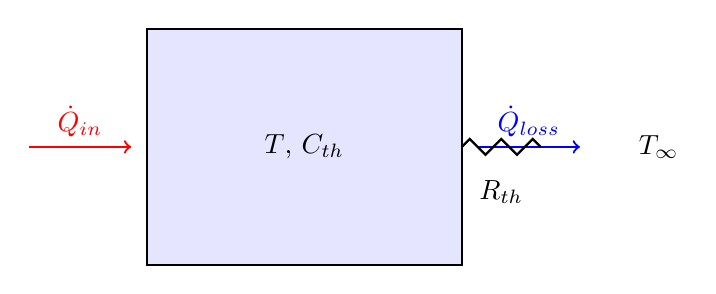
\begin{tikzpicture}
    % Room/body
    \draw[thick, fill=blue!10] (0,0) rectangle (4,3);
    \node at (2,1.5) {$T$, $C_{th}$};

    % Heater input
    \draw[->, thick, red] (-1.5,1.5) -- (-0.2,1.5) node[above, midway] {$\dot{Q}_{\text{in}}$};

    % Heat loss
    \draw[->, thick, blue] (4.2,1.5) -- (5.5,1.5) node[above, midway] {$\dot{Q}_{\text{loss}}$};

    % Ambient
    \node at (6.5,1.5) {$T_\infty$};

    % Thermal resistance
    \draw[thick, decorate, decoration={zigzag, segment length=4mm, amplitude=1mm}]
        (4,1.5) -- (5,1.5);
    \node[below] at (4.5,1.2) {$R_{th}$};
\end{tikzpicture}
\caption{Single-capacitance thermal system.}
\label{fig:single_thermal}
\end{figure}


Energy balance:
\begin{equation}
C_{th}\frac{\dd T}{\dd t} = \dot{Q}_{\text{in}} - \frac{T - T_\infty}{R_{th}}
\end{equation}

where $C_{th} = mC_p$ is the thermal capacitance.

Rearranging:
\begin{equation}
\boxed{R_{th}C_{th}\frac{\dd T}{\dd t} + T = R_{th}\dot{Q}_{\text{in}} + T_\infty}
\end{equation}

\subsection{Transfer Function}

Defining $\theta = T - T_\infty$ (temperature above ambient):
\begin{equation}
G(s) = \frac{\Theta(s)}{\dot{Q}_{\text{in}}(s)} = \frac{R_{th}}{\tau s + 1}
\end{equation}

where $\tau = R_{th}C_{th}$ is the thermal time constant.

\begin{examplebox}[title=Example 1.10: Room Heating]
A room has thermal capacitance $C_{th} = 500$ kJ/K and thermal resistance to outdoors $R_{th} = 0.01$ K/W. Find:
\begin{enumerate}[label=(\alph*)]
    \item The thermal time constant
    \item The heater power needed to maintain 20°C when outdoor temperature is 0°C
    \item The room temperature 1 hour after turning off the heater
\end{enumerate}

\textbf{Solution:}

(a) Time constant:
\begin{equation}
\tau = R_{th}C_{th} = 0.01 \times 500{,}000 = 5000 \text{ s} = 83.3 \text{ min}
\end{equation}

(b) Steady-state heat balance:
\begin{equation}
\dot{Q}_{\text{in}} = \frac{T - T_\infty}{R_{th}} = \frac{20 - 0}{0.01} = 2000 \text{ W} = 2 \text{ kW}
\end{equation}

(c) After heater off (cooling from 20°C):
\begin{equation}
T(t) = T_\infty + (T_0 - T_\infty)\ee^{-t/\tau} = 0 + 20\ee^{-3600/5000} = 9.7°\text{C}
\end{equation}
\end{examplebox}

% ============================================================================
\section{Multi-Capacitance Thermal Systems}
\label{sec:multi_thermal}
% ============================================================================

\begin{figure}[htbp]
\centering
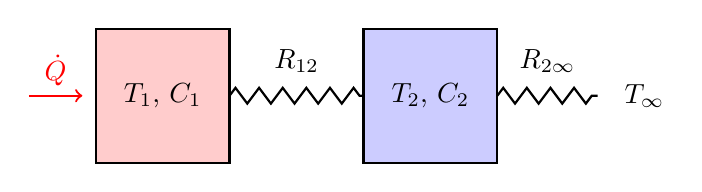
\begin{tikzpicture}[scale=0.85]
    % Body 1
    \draw[thick, fill=red!20] (0,0) rectangle (2,2);
    \node at (1,1) {$T_1$, $C_1$};

    % Body 2
    \draw[thick, fill=blue!20] (4,0) rectangle (6,2);
    \node at (5,1) {$T_2$, $C_2$};

    % Resistance between
    \draw[thick, decorate, decoration={zigzag, segment length=3mm, amplitude=1mm}]
        (2,1) -- (4,1);
    \node[above] at (3,1.2) {$R_{12}$};

    % Heat input
    \draw[->, thick, red] (-1,1) -- (-0.2,1) node[above, midway] {$\dot{Q}$};

    % Heat loss from body 2
    \draw[thick, decorate, decoration={zigzag, segment length=3mm, amplitude=1mm}]
        (6,1) -- (7.5,1);
    \node[above] at (6.75,1.2) {$R_{2\infty}$};
    \node at (8.2,1) {$T_\infty$};
\end{tikzpicture}
\caption{Two-capacitance thermal system.}
\label{fig:two_thermal}
\end{figure}


Energy balances:
\begin{align}
C_1\frac{\dd T_1}{\dd t} &= \dot{Q} - \frac{T_1 - T_2}{R_{12}} \\
C_2\frac{\dd T_2}{\dd t} &= \frac{T_1 - T_2}{R_{12}} - \frac{T_2 - T_\infty}{R_{2\infty}}
\end{align}

This yields a second-order system with two thermal time constants.

% ============================================================================
\section{Fluid Systems: Tank Level}
\label{sec:tank_level}
% ============================================================================

\begin{figure}[htbp]
\centering
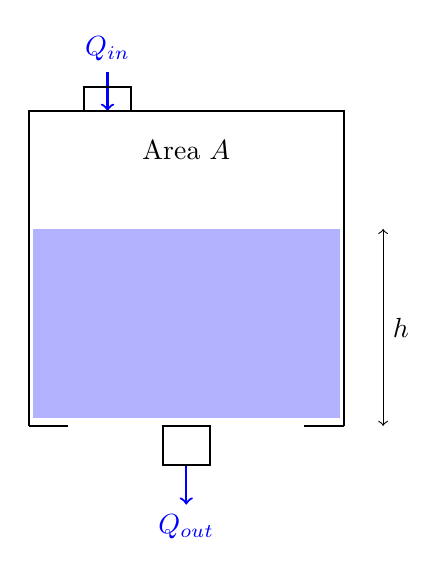
\begin{tikzpicture}
    % Tank
    \draw[thick] (0,0) -- (0,4) -- (4,4) -- (4,0);
    \draw[thick] (0,0) -- (0.5,0) (3.5,0) -- (4,0);

    % Liquid
    \fill[blue!30] (0.05,0.1) rectangle (3.95,2.5);

    % Level
    \draw[<->] (4.5,0) -- (4.5,2.5) node[midway, right] {$h$};

    % Inflow
    \draw[->, thick, blue] (1,4.5) -- (1,4) node[above, pos=0] {$Q_{\text{in}}$};
    \draw[thick] (0.7,4) rectangle (1.3,4.3);

    % Outflow
    \draw[->, thick, blue] (2,-0.5) -- (2,-1) node[below] {$Q_{\text{out}}$};
    \draw[thick] (1.7,-0.5) rectangle (2.3,0);

    % Area
    \node at (2,3.5) {Area $A$};
\end{tikzpicture}
\caption{Single tank level system.}
\label{fig:tank_level}
\end{figure}


\subsection{Mass Balance}

For incompressible fluid:
\begin{equation}
A\frac{\dd h}{\dd t} = Q_{\text{in}} - Q_{\text{out}}
\end{equation}

\subsection{Outflow Models}

\subsubsection{Linear resistance (laminar flow through valve)}
\begin{equation}
Q_{\text{out}} = \frac{h}{R_f}
\end{equation}

where $R_f$ is the fluid resistance.

\subsubsection{Nonlinear resistance (turbulent flow, orifice)}
\begin{equation}
Q_{\text{out}} = C_d A_o \sqrt{2gh}
\end{equation}

This is nonlinear but can be linearized about an operating point.

\subsection{Linear Tank Model}

With linear resistance:
\begin{equation}
A\frac{\dd h}{\dd t} + \frac{h}{R_f} = Q_{\text{in}}
\end{equation}

Transfer function:
\begin{equation}
G(s) = \frac{H(s)}{Q_{\text{in}}(s)} = \frac{R_f}{\tau s + 1}
\end{equation}

where $\tau = AR_f$ is the hydraulic time constant.

\begin{examplebox}[title=Example 1.11: Water Tank]
A cylindrical tank has diameter 2 m and drains through a valve with resistance $R_f = 100$ s/m$^2$. Find:
\begin{enumerate}[label=(\alph*)]
    \item The time constant
    \item Steady-state level for inflow of 0.01 m$^3$/s
    \item Time to reach 90\% of steady-state from empty
\end{enumerate}

\textbf{Solution:}

Tank area: $A = \pi(1)^2 = 3.14$ m$^2$

(a) Time constant:
\begin{equation}
\tau = AR_f = 3.14 \times 100 = 314 \text{ s} = 5.2 \text{ min}
\end{equation}

(b) Steady-state level:
\begin{equation}
h_{ss} = R_f \times Q_{\text{in}} = 100 \times 0.01 = 1 \text{ m}
\end{equation}

(c) Time to 90\%:
\begin{equation}
0.9 = 1 - \ee^{-t/\tau} \implies t = -\tau\ln(0.1) = 314 \times 2.3 = 723 \text{ s} = 12 \text{ min}
\end{equation}
\end{examplebox}

% ============================================================================
\section{Interacting Tank Systems}
\label{sec:interacting_tanks}
% ============================================================================

\begin{figure}[htbp]
\centering
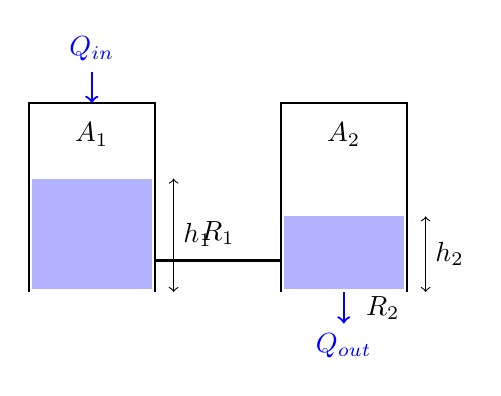
\begin{tikzpicture}[scale=0.8]
    % Tank 1
    \draw[thick] (0,0) -- (0,3) -- (2,3) -- (2,0);
    \fill[blue!30] (0.05,0.05) rectangle (1.95,1.8);
    \node at (1,2.5) {$A_1$};
    \draw[<->] (2.3,0) -- (2.3,1.8) node[midway, right] {$h_1$};

    % Tank 2
    \draw[thick] (4,0) -- (4,3) -- (6,3) -- (6,0);
    \fill[blue!30] (4.05,0.05) rectangle (5.95,1.2);
    \node at (5,2.5) {$A_2$};
    \draw[<->] (6.3,0) -- (6.3,1.2) node[midway, right] {$h_2$};

    % Connecting pipe
    \draw[thick] (2,0.5) -- (4,0.5);
    \node[above] at (3,0.6) {$R_1$};

    % Inflow
    \draw[->, thick, blue] (1,3.5) -- (1,3) node[above, pos=0] {$Q_{\text{in}}$};

    % Outflow
    \draw[->, thick, blue] (5,0) -- (5,-0.5) node[below] {$Q_{\text{out}}$};
    \node[right] at (5.2,-0.25) {$R_2$};
\end{tikzpicture}
\caption{Two interacting tanks.}
\label{fig:two_tanks}
\end{figure}


Mass balances:
\begin{align}
A_1\frac{\dd h_1}{\dd t} &= Q_{\text{in}} - \frac{h_1 - h_2}{R_1} \\
A_2\frac{\dd h_2}{\dd t} &= \frac{h_1 - h_2}{R_1} - \frac{h_2}{R_2}
\end{align}

This is a second-order system. The interaction between tanks creates coupling that affects the system dynamics.

% ============================================================================
\section{Hydraulic Actuators}
\label{sec:hydraulic}
% ============================================================================

\begin{figure}[htbp]
\centering
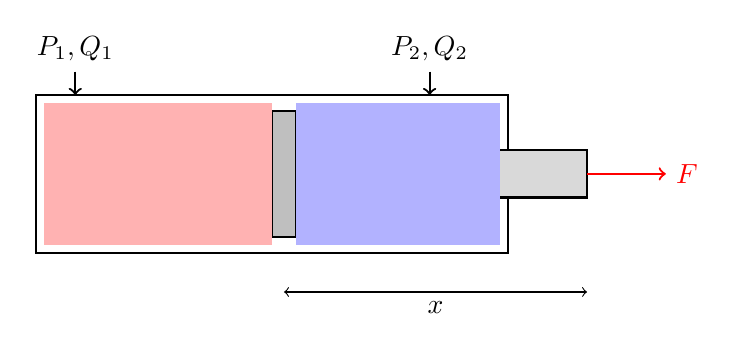
\begin{tikzpicture}
    % Cylinder
    \draw[thick] (0,0) rectangle (6,2);

    % Piston
    \draw[thick, fill=gray!50] (3,0.2) rectangle (3.3,1.8);

    % Rod
    \draw[thick, fill=gray!30] (3.3,0.7) rectangle (7,1.3);

    % Chambers
    \fill[red!30] (0.1,0.1) rectangle (3,1.9);
    \fill[blue!30] (3.3,0.1) rectangle (5.9,1.9);

    % Ports
    \draw[->, thick] (0.5,2.3) -- (0.5,2) node[above, pos=0] {$P_1, Q_1$};
    \draw[->, thick] (5,2.3) -- (5,2) node[above, pos=0] {$P_2, Q_2$};

    % Displacement
    \draw[<->] (3.15,-0.5) -- (7,-0.5) node[midway, below] {$x$};

    % Force
    \draw[->, thick, red] (7,1) -- (8,1) node[right] {$F$};
\end{tikzpicture}
\caption{Double-acting hydraulic cylinder.}
\label{fig:hydraulic_cylinder}
\end{figure}


\subsection{Flow Continuity}

For incompressible fluid:
\begin{equation}
Q_1 = A_1\dot{x} + \frac{V_1}{\beta}\dot{P}_1
\end{equation}

where $\beta$ is the bulk modulus.

\subsection{Force Balance}

\begin{equation}
M\ddot{x} = P_1 A_1 - P_2 A_2 - F_{\text{load}} - B\dot{x}
\end{equation}

\subsection{Servo Valve Model}

Flow through a servo valve:
\begin{equation}
Q = C_d w x_v \sqrt{\frac{2(P_s - P_L)}{\rho}}
\end{equation}

where $x_v$ is the valve spool position.

Linearized about operating point:
\begin{equation}
Q = K_q x_v - K_c P_L
\end{equation}

% ============================================================================
\section{Pneumatic Systems}
\label{sec:pneumatic}
% ============================================================================

Pneumatic systems use compressible gas (usually air), adding complexity:

\subsubsection{Ideal gas law}
\begin{equation}
PV = mRT
\end{equation}

\subsubsection{Mass flow through orifice}

For subsonic flow ($P_2/P_1 > 0.528$):
\begin{equation}
\dot{m} = C_d A P_1 \sqrt{\frac{2}{RT_1}} \sqrt{\frac{\gamma}{\gamma-1}\left[\left(\frac{P_2}{P_1}\right)^{2/\gamma} - \left(\frac{P_2}{P_1}\right)^{(\gamma+1)/\gamma}\right]}
\end{equation}

For choked flow ($P_2/P_1 \leq 0.528$):
\begin{equation}
\dot{m} = C_d A P_1 \sqrt{\frac{\gamma}{RT_1}}\left(\frac{2}{\gamma+1}\right)^{(\gamma+1)/(2(\gamma-1))}
\end{equation}

\subsection{Pneumatic Cylinder}

Pressure dynamics in chamber:
\begin{equation}
\frac{\dd P}{\dd t} = \frac{\gamma R T}{V}(\dot{m}_{\text{in}} - \dot{m}_{\text{out}}) - \frac{\gamma P}{V}\dot{V}
\end{equation}

% ============================================================================
\section{Heat Exchangers}
\label{sec:heat_exchanger}
% ============================================================================

\begin{figure}[htbp]
\centering
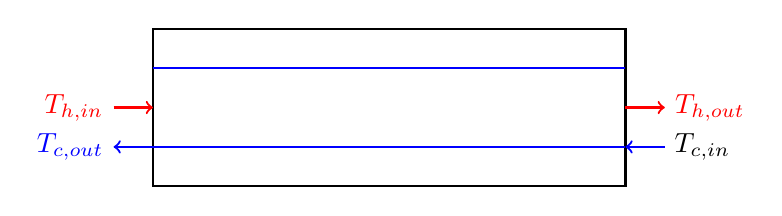
\begin{tikzpicture}
    % Shell
    \draw[thick] (0,0) rectangle (6,2);

    % Tubes (simplified)
    \draw[thick, blue] (0,0.5) -- (6,0.5);
    \draw[thick, blue] (0,1.5) -- (6,1.5);

    % Hot fluid
    \draw[->, thick, red] (-0.5,1) -- (0,1) node[left, pos=0] {$T_{h,\text{in}}$};
    \draw[->, thick, red] (6,1) -- (6.5,1) node[right] {$T_{h,\text{out}}$};

    % Cold fluid
    \draw[->, thick, blue] (6.5,0.5) -- (6,0.5);
    \draw[->, thick, blue] (0,0.5) -- (-0.5,0.5) node[left] {$T_{c,\text{out}}$};
    \node[right] at (6.5,0.5) {$T_{c,\text{in}}$};
\end{tikzpicture}
\caption{Counter-flow heat exchanger.}
\label{fig:heat_exchanger}
\end{figure}


Simplified lumped model:
\begin{align}
C_h\frac{\dd T_h}{\dd t} &= \dot{m}_h c_{p,h}(T_{h,\text{in}} - T_h) - UA(T_h - T_c) \\
C_c\frac{\dd T_c}{\dd t} &= \dot{m}_c c_{p,c}(T_{c,\text{in}} - T_c) + UA(T_h - T_c)
\end{align}

where $UA$ is the overall heat transfer coefficient times area.

% ============================================================================
\section{Thermal Resistance Networks}
\label{sec:thermal_resistance_network}
% ============================================================================

\begin{figure}[htbp]
\centering
\begin{tikzpicture}[scale=1.0]
    % Title area
    \node at (3.5, 5.2) {\textbf{Series Thermal Resistance Network}};

    % Heat source
    \draw[fill=UofSCGarnet!30] (0,4) rectangle (0.6,4.6);
    \node[color=UofSCBlack] at (0.3,4.3) {$\dot{Q}$};

    % Resistance 1 (zigzag)
    \draw[thick, decorate, decoration={zigzag, segment length=3mm, amplitude=0.6mm}]
        (0.8,4.3) -- (1.8,4.3);
    \node[above] at (1.3,4.5) {$R_1$};

    % Node 1
    \node[circle, draw=UofSCBlack, fill=UofSCAtlantic!20, minimum size=0.4cm] at (2.2,4.3) {};
    \node[below] at (2.2,3.9) {$T_1$, $C_1$};

    % Resistance 2 (zigzag)
    \draw[thick, decorate, decoration={zigzag, segment length=3mm, amplitude=0.6mm}]
        (2.6,4.3) -- (3.6,4.3);
    \node[above] at (3.1,4.5) {$R_2$};

    % Node 2
    \node[circle, draw=UofSCBlack, fill=UofSCAtlantic!20, minimum size=0.4cm] at (4,4.3) {};
    \node[below] at (4,3.9) {$T_2$, $C_2$};

    % Resistance 3 (zigzag) - to ambient
    \draw[thick, decorate, decoration={zigzag, segment length=3mm, amplitude=0.6mm}]
        (4.4,4.3) -- (5.4,4.3);
    \node[above] at (4.9,4.5) {$R_3$};

    % Ambient
    \node at (6,4.3) {$T_\infty$};

    % Parallel configuration below
    \node at (3.5, 2.8) {\textbf{Parallel Thermal Paths}};

    % Main node
    \node[circle, draw=UofSCBlack, fill=UofSCAtlantic!20, minimum size=0.5cm] at (2,1.8) {};
    \node[below] at (2,1.25) {$T_c$, $C_c$};

    % Path 1 (upper)
    \draw[thick, decorate, decoration={zigzag, segment length=2.5mm, amplitude=0.5mm}]
        (2.25,2.15) -- (3.5,2.15);
    \node[above] at (2.9,2.35) {$R_{c1}$};
    \node at (4.2,2.15) {$T_\infty$};

    % Path 2 (lower)
    \draw[thick, decorate, decoration={zigzag, segment length=2.5mm, amplitude=0.5mm}]
        (2.25,1.45) -- (3.5,1.45);
    \node[below] at (2.9,1.25) {$R_{c2}$};
    \node at (4.2,1.45) {$T_\infty$};

    % Input to main node
    \draw[->, thick, UofSCGarnet] (0.5,1.8) -- (1.3,1.8);
    \node[above] at (0.9,1.95) {$\dot{Q}_{\text{in}}$};
\end{tikzpicture}
\caption{Thermal resistance networks showing series (top) and parallel (bottom) heat flow paths with thermal capacitances at nodes.}
\label{fig:thermal_resistance_network}
\end{figure}


\subsection{Network Analysis}

For \textbf{series resistances}, the total thermal resistance equals the sum:
\begin{equation}
R_{\text{total}} = R_1 + R_2 + R_3 + \cdots
\end{equation}

The heat flow through all resistances is identical (same current). The temperature difference across each resistance is proportional to its value.

For \textbf{parallel resistances}, the equivalent resistance is:
\begin{equation}
\frac{1}{R_{\text{eq}}} = \frac{1}{R_{c1}} + \frac{1}{R_{c2}} + \cdots
\end{equation}

Each path dissipates heat proportionally to the inverse of its resistance. Parallel paths reduce the effective resistance, increasing heat flow.

% ============================================================================
\section{Two-Tank Fluid System Dynamics}
\label{sec:two_tank_dynamics}
% ============================================================================

\begin{figure}[htbp]
\centering
\begin{tikzpicture}[scale=0.9]
    % Tank 1
    \draw[thick, UofSCBlack] (0,0) -- (0,5) -- (3,5) -- (3,0);
    \fill[UofSCAtlantic!15] (0.1,0.1) rectangle (2.9,3);

    % Tank 1 level indicator
    \draw[<->, thick, UofSCHorseshoe] (3.3,0) -- (3.3,3);
    \node[right, UofSCHorseshoe] at (3.5,1.5) {$h_1$};
    \node at (1.5,4.3) {\textbf{Tank 1}};
    \node[small] at (1.5,3.8) {$A_1$};

    % Tank 2
    \draw[thick, UofSCBlack] (5,0) -- (5,4) -- (8,4) -- (8,0);
    \fill[UofSCAtlantic!15] (5.1,0.1) rectangle (7.9,2);

    % Tank 2 level indicator
    \draw[<->, thick, UofSCHorseshoe] (8.3,0) -- (8.3,2);
    \node[right, UofSCHorseshoe] at (8.5,1) {$h_2$};
    \node at (6.5,3.3) {\textbf{Tank 2}};
    \node[small] at (6.5,2.8) {$A_2$};

    % Inflow to Tank 1
    \draw[->, thick, UofSCCongaree] (1.5,5.5) -- (1.5,5);
    \node[above, UofSCCongaree] at (1.5,5.6) {$Q_{\text{in}}$};

    % Connection between tanks (valve)
    \draw[thick, UofSCBlack] (3,1.5) -- (5,1.5);
    \draw[thick, UofSCHoneycomb, fill=UofSCHoneycomb!30] (3.8,1.2) rectangle (4.2,1.8);
    \node[below, small] at (4,0.9) {$R_1$};

    % Flow from tank 1 to tank 2
    \draw[->, thick, UofSCCongaree] (3.5,1.5) -- (4.5,1.5);
    \node[above, UofSCCongaree, small] at (4,1.7) {$Q_{12}$};

    % Outflow from Tank 2
    \draw[->, thick, UofSCCongaree] (6.5,-0.5) -- (6.5,-1.2);
    \node[below, UofSCCongaree] at (6.5,-1.3) {$Q_{\text{out}}$};

    % Outlet valve
    \draw[thick, UofSCHoneycomb, fill=UofSCHoneycomb!30] (6.3,-0.2) rectangle (6.7,0.2);
    \node[right, small] at (7,0) {$R_2$};

    % Equations box
    \draw[thick, UofSCAtlantic, dash pattern=on 2pt off 2pt] (0,-2.2) rectangle (8,-1);
    \node[anchor=west, small] at (0.2,-1.3) {$A_1\frac{dh_1}{dt} = Q_{\text{in}} - \frac{h_1 - h_2}{R_1}$};
    \node[anchor=west, small] at (0.2,-1.8) {$A_2\frac{dh_2}{dt} = \frac{h_1 - h_2}{R_1} - \frac{h_2}{R_2}$};
\end{tikzpicture}
\caption{Two-tank fluid system showing mass conservation, inter-tank flow through resistance $R_1$, and outflow through $R_2$. Shaded regions indicate liquid level.}
\label{fig:two_tank_system}
\end{figure}


This configuration creates a second-order system where tank interactions cause non-minimum-phase behavior. The inter-tank resistance $R_1$ introduces coupling between the tanks.

% ============================================================================
\section{Exercises: Thermal and Fluid Systems}
% ============================================================================

\begin{exercise}
A metal block ($m = 5$ kg, $C_p = 500$ J/kg$\cdot$K) is heated by a 100 W heater and loses heat to 25°C ambient through convection ($hA = 5$ W/K).
\begin{enumerate}[label=(\alph*)]
    \item Write the differential equation for block temperature
    \item Find the thermal time constant
    \item Find the steady-state temperature
    \item How long to reach 90\% of steady-state from ambient?
\end{enumerate}
\end{exercise}

\begin{exercise}
\textbf{Thermal Resistance Network:} A system has two thermal resistances in series: $R_1 = 0.5$ K/W and $R_2 = 0.8$ K/W, with a heat source $\dot{Q} = 500$ W and ambient temperature $T_\infty = 20$°C. The total thermal capacitance is $C_{th} = 10$ kJ/K.
\begin{enumerate}[label=(\alph*)]
    \item Find the total thermal resistance
    \item Find the steady-state temperature rise above ambient
    \item If the system starts at ambient, find the temperature after 100 seconds
\end{enumerate}
\end{exercise}

\begin{exercise}
Two tanks in series each have $A = 1$ m$^2$. The first tank drains into the second through resistance $R_1 = 50$ s/m$^2$, and the second drains to atmosphere through $R_2 = 100$ s/m$^2$.
\begin{enumerate}[label=(\alph*)]
    \item Write the state-space model
    \item Find the transfer function from $Q_{\text{in}}$ to $h_2$
    \item Find the system poles and time constants
    \item Explain how the inter-tank interaction affects the response
\end{enumerate}
\end{exercise}

\begin{exercise}
\textbf{Tank Level Dynamics:} A conical tank has height-dependent area: $A(h) = \pi(rh/H)^2$ where $r = 0.5$ m is base radius and $H = 2$ m is total height. The outlet has resistance $R_f = 80$ s/m$^2$.
\begin{enumerate}[label=(\alph*)]
    \item Write the nonlinear ODE for level $h$
    \item For $h = 1$ m at steady-state with constant inflow, find $Q_{\text{in}}$
    \item Linearize the model about this operating point
\end{enumerate}
\end{exercise}

\begin{exercise}
A hydraulic servo system has a 10 cm diameter piston, 1000 kg load mass, and bulk modulus $\beta = 1.5 \times 10^9$ Pa. The chamber volume is 0.5 L.
\begin{enumerate}[label=(\alph*)]
    \item Calculate the hydraulic natural frequency
    \item If damping ratio is 0.3, find the damping coefficient
    \item Sketch the expected step response
\end{enumerate}
\end{exercise}

\begin{exercise}
\textbf{Heat Exchanger Thermal Dynamics:} A counter-flow heat exchanger receives hot fluid at 80°C (inlet) with flow rate 0.5 kg/s, and cold fluid at 20°C with flow rate 0.3 kg/s. The heat transfer coefficient is $UA = 2$ kW/K, and thermal capacitances are $C_h = C_c = 5$ kJ/K.
\begin{enumerate}[label=(\alph*)]
    \item Write the energy balance equations for both sides
    \item Find the steady-state outlet temperatures
    \item Determine the time constants of the hot and cold sides
\end{enumerate}
\end{exercise}

\begin{exercise}
A hot water tank ($V = 200$ L) receives water at 15°C at rate 0.1 L/s and has a 3 kW heater. Heat loss to ambient is $UA = 10$ W/K. Find the steady-state temperature and time constant. What is the response time to reach 95\% of steady-state?
\end{exercise}
